\documentclass[./main.tex]{subfiles}

\begin{document}
\begin{figure}[t]
    \centering
    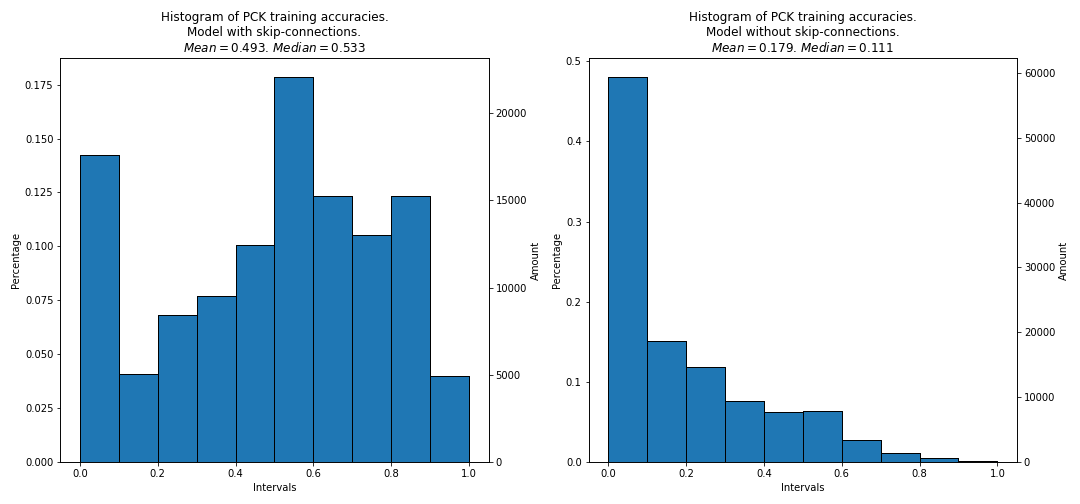
\includegraphics[height = 6 cm]{entities/PCK_accs_vs.png}
    \caption{Histogram of PCK training accuracies of the model with the skip-connections enabled (left) and the model with the skip connections disabled (right).}
    \label{fig:PCK_accs}
\end{figure}

\section{Understanding the Model}\label{sec:XAI}
In the following section we will be interpreting the model developed in section \ref{experiement}, with the intention of getting an understanding of how the model works.

\subsection{Motivation}
Deep learning models are often complex and work like a \textit{black boxes}. By that it is meant, that when a network is given some input, the model simply just returns some output without any explanation or reasoning behind the output. This can often be a problem, especially in cases where the output of the network can result in a life or death situation of a human. For that reason, understanding and explaining how a network works can be very important - this is what is called \textit{explainable ai} (\textit{XAI}) 
\\
\\
Selvaraju \textit{et al.} \cite{Selvaraju} argues that there are three cases for using explainable ai:
\begin{enumerate}
    \item When the network performs worse than humans, an understanding of the network can help us improve the performance of the model.
    \item When the network is on par with humans, an understanding of the network is trivial for humans to build trust in the network, as we can understand its strengths and weaknesses
    \item When the network performs better than humans, an understanding of the network can teach humans how to perform better.
\end{enumerate}
Throughout section \ref{sec:XAI} we will be getting an understanding of our model developed in section \ref{experiement}, as we wish to understand its strengths and weaknesses.
% MÅSKE OGSÅ, AT VI VIL FORBEDRE MODELLEN!

\subsection{Verifying the Effects of Skip-Connections}\label{subsec:verifying_skip_cons}
Olsen \cite{Camilla} and Newell \cite{Newell} claims, that the skip-connections are used in order to recreate details that are lost during the encoder-phase. Throughout subsection \ref{subsec:verifying_skip_cons} we will be verifying or refuting the claim of the effect of the skip-connections. To do so we will be using two models based on the same network:
\begin{enumerate}
    \item The trained Stacked Hourglass from section \ref{experiement}
    \item The trained Stacked Hourglass from section \ref{experiement}, but with the skip-connections disabled.
\end{enumerate}
Thus, the second model has not been retrained and is identical to the first model, however, without its skip-connections.
\\
\\
In Figure \ref{fig:PCK_accs} the distributions of the PCK training accuracies of the two models have been visualized. We have decided to make use of the training data for computing the PCK accuracies, as we want to look at the data, that the model has been trained on. By looking at the two distributions we can clearly see, how to model without its skip-connections performs much worse, than the model with its skip-connections.
\\
\\
To further understand the decrease of accuracy in the case where the skip-connections are disabled, we have in Figure \ref{fig:pred_comparison} visualized $20$ samples from the training dataset, where the model with skip-connections has an $100\%$ PCK accuracy score. Next to each image the ground truth heatmaps, or the prediction by the model with skip-connections, and the prediction by the model without skip-connections has been visualized.
\\
\begin{figure}[p]
    \centering
    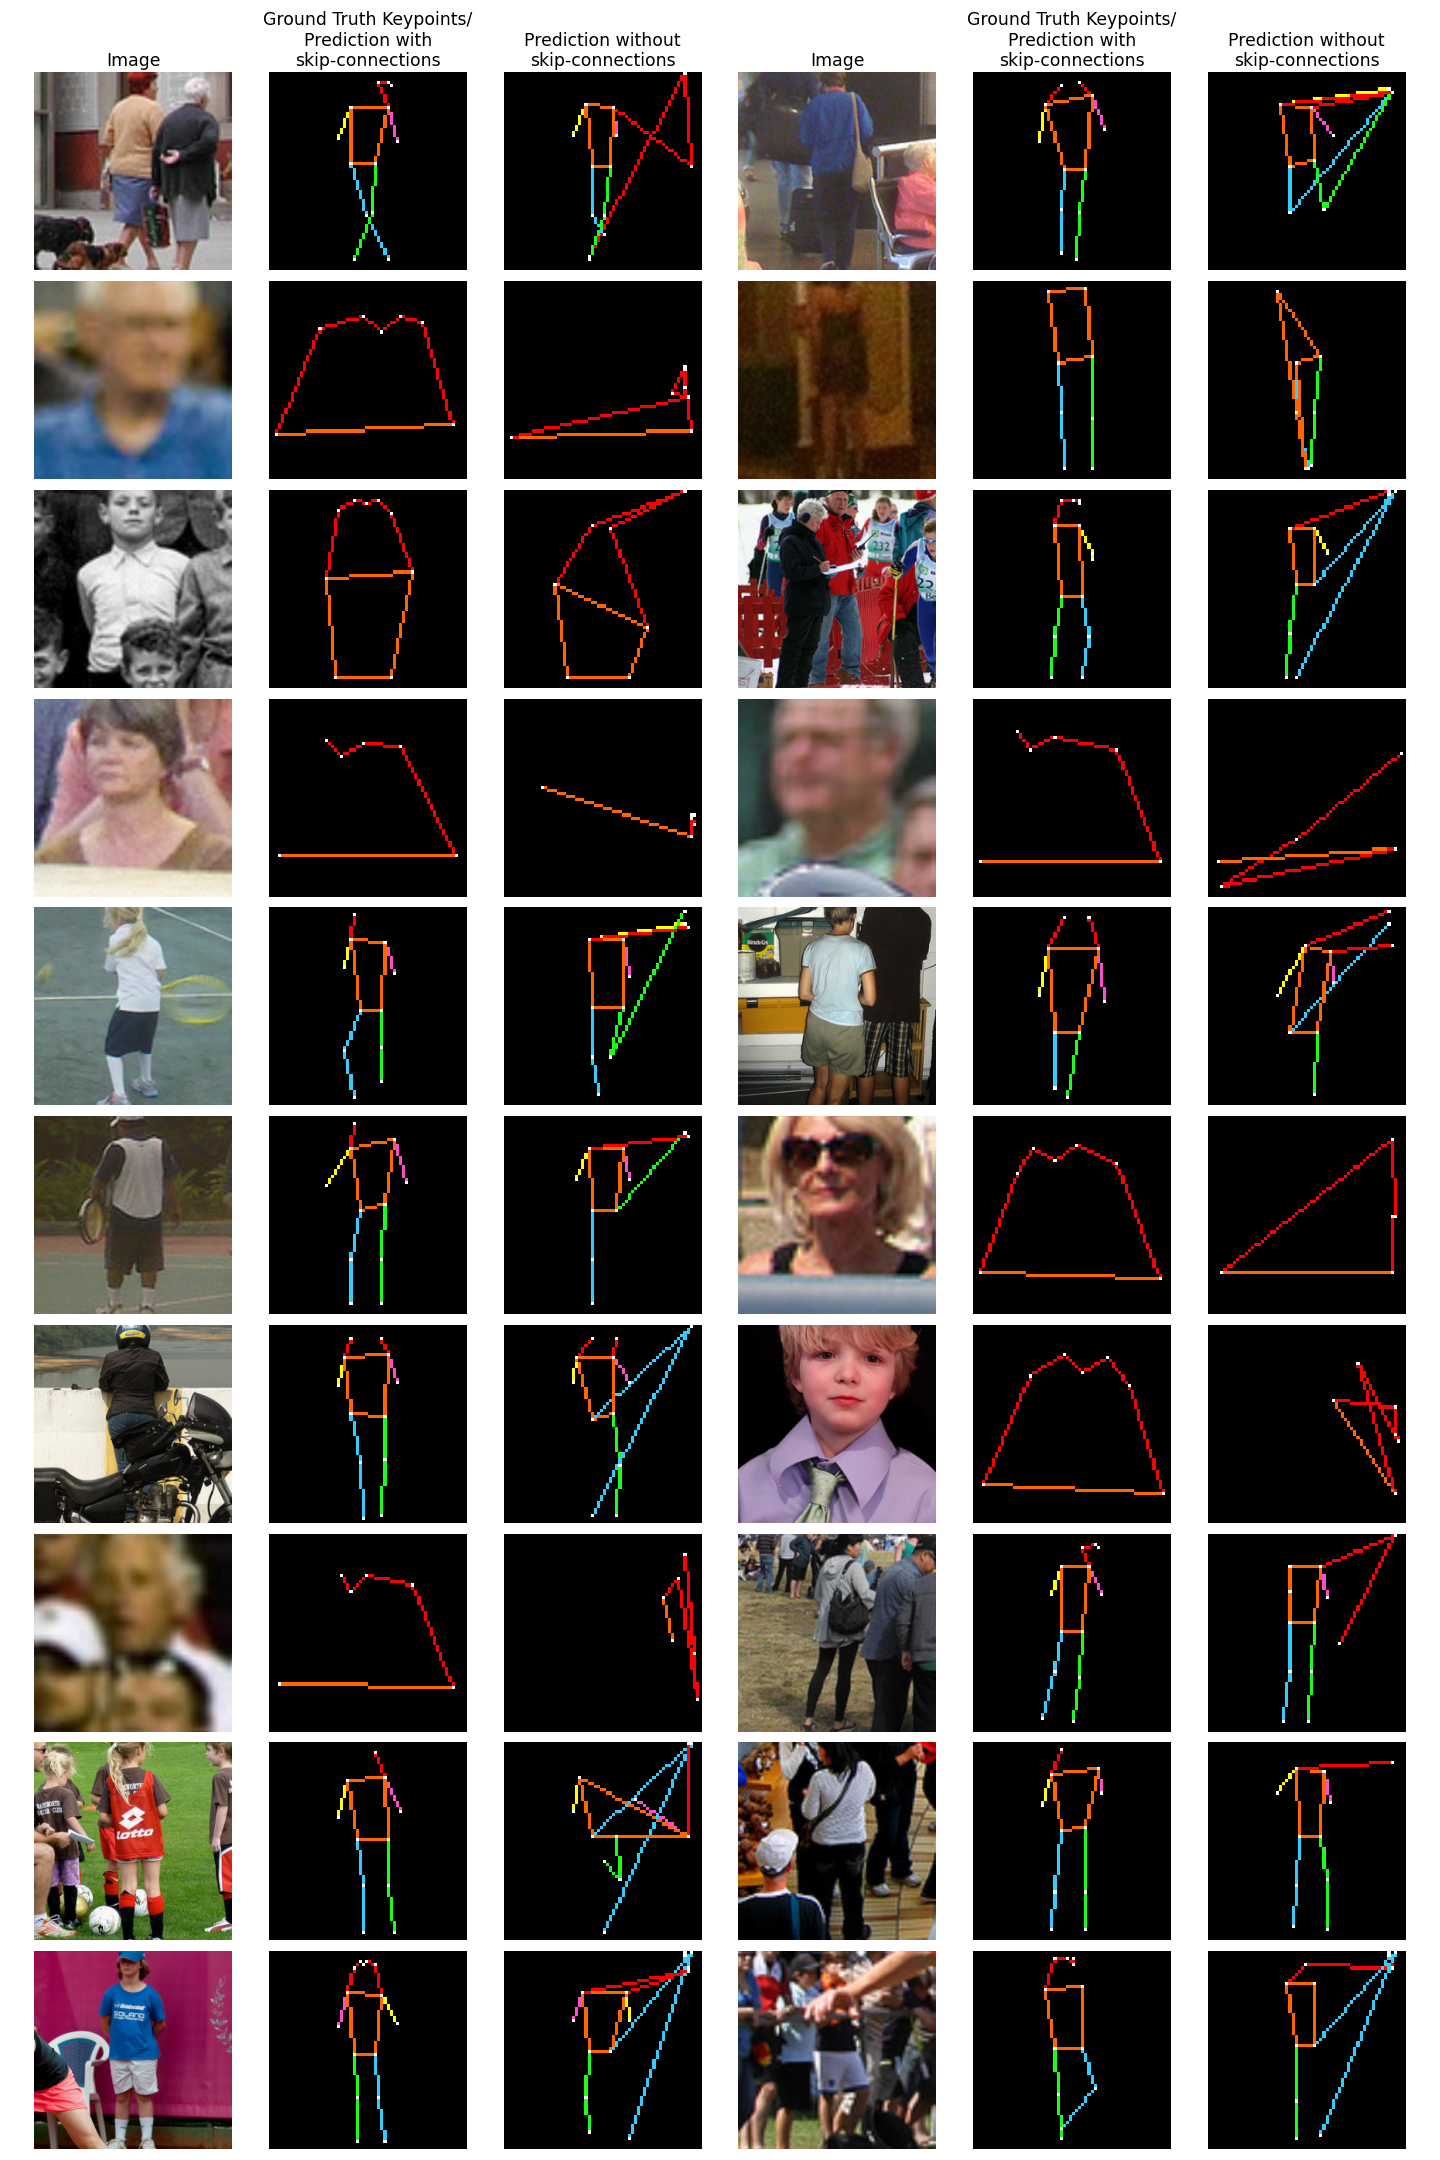
\includegraphics[width = \textwidth]{entities/pred_comparisons.png}
    \caption{20 samples of images correctly predicted by the model with skip-connections enabled, the corresponding ground truth heatmap and predictions by the model with skip-connections disabled.}
    \label{fig:pred_comparison}
\end{figure}
\\
By looking at Figure \ref{fig:pred_comparison} we can see, that the model without its skip-connections often struggles with smaller joints, such as the eyes, ears or nose, whereas it performs better, however still not always perfect, on bigger joints, such as the shoulders, hips or knees. This is probably due to the fact, that the details of the smaller joints has a bigger chance of being lost by the max pooling layers in the encoder. Without the skip-connections they are thus not recreatable in the decoder, resulting in bad predictions. Thus, we can verify Olsen's \cite{Camilla} and Newell's \cite{Newell} claims, that the skip-connections are used for recreating details lost in the encoder. 


\subsection{Shape Analysis of the Latent Space}


\subsection{Using Clustering to Seperate the Latent Space}

\end{document}